\chapter{Preliminaries}\label{chap:preliminaries}

This section formalises necessary ingredients and the~problem statement for probabilistic synthesis.
We will first introduce a~discrete-time Markov chain as the~simplest operation model for probabilistic programs.
Further,~we will describe a~Markov decision process representing a~similar model as a~Markov chain,~but it contains additional non-determinism.
These models play a~crucial role when synthesising probabilistic programs,~as we will see later in Chapter~\ref{chap:synthesis_methods}.
The~following definitions are inspired from the~existing sources,~mainly from~\cite{tacas21,Quatmann2016},~where a~more detailed description can also be found.

\section{Probabilistic Models}

% \MC{Navrhuju napsat nejakou uvodni vetu, ze MC je semantika prob programu a podobne trochu nize ze MDP nam dovoluji uvazovat o mnozine prog programu.}
We denote a~finite set of \textit{parameters} as $V$.
We consider \textit{parameters} over the~domain $\real$ ranged over by $x,y,z$ for the~following definitions.
Let $u: V \rightarrow \real$ denote a~\textit{valuation} for \textit{parameters} $V$.
We denote a~set of \textit{multi-affine multivariate polynomials} as $\mathbb{Q}_V$, where polynomial $f$ is defined over parameters $V$ and equal to $\sum_{i \leq M}{\prod_{v\in V_i}v \cdot a_i}$,~for appropriate $M \in \nat$, $a_i \in \rat$,~and $\forall \, 0 \leq i \leq m. \; V_i \subseteq V$.
We note that this set includes only the polynomials where the~variables have the~maximal degree equal to one,~i.e.,~$y^3 \notin \mathbb{Q}_V$, but $y \cdot z \in \mathbb{Q}_V$.
When we apply the~valuation $u$ to polynomial $f \in \mathbb{Q}_V$,~the~resulting instance yields a~real number $f[u] \in \real$,~in which all occurrences of variable $x \in f$ are replaced by $u(x)$.
We consider various types of (parametric) discrete probabilistic models.
We can look at them as the~transition systems with the~given state space where the~transitions are marked with polynomials in $\mathbb{Q}_V$~\cite{Quatmann2016}.

\begin{definition}[pMDP]
A parametric Markov decision process (pMDP) $\mathcal{M}$ is a tuple $(S, V, s_0, Act, \mathcal{P})$, where $S$ is a finite set of states, $V$ is a finite set of parameters over $\real$, $s_0 \in S$ is an initial state, $Act$ is a non-empty finite set of actions, and $\mathcal{P}: S \times Act  \times S \nrightarrow \mathbb{Q}_V$ is a transition function.
\end{definition}
A~set $\mathit{Act(s) = \{ a \in Act \; \lvert \; \exists s' \in S. \mathcal{P}(s, a, s') \neq \; \perp \}}$ for state $s \in S$ represents the~\textit{available} actions.
The~model do not contains deadlock states,~since for each state $s \in S$ holds that the~action set $Act(s)$ is non-empty.
When holds $\lvert \mathit{Act(s)} \rvert = 1$ for each state $s \in S$,~such pMDP straightforward induces an~parametric Markov chain (pMC),~which has enabled only one action at each state.

\begin{figure*}[h!]
\centering
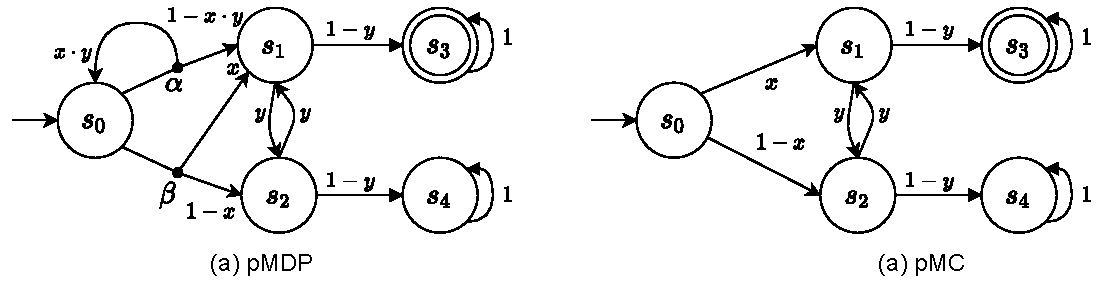
\includegraphics[width=1.0\textwidth]{figures/param_models.pdf}
\caption{The introduced kinds of parametric probabilistic models \,--\, pMDP and pMC.}%
\label{fig:param_models}%
\end{figure*}

\begin{example}[Parametric models]
We depict (a) pMDP and (b) pMC with parameters $\{x, y\}$ at Figure~\ref{fig:param_models}.
We mark an~initial state $s_0 \in S$  with an~arrow,~and the~target state $s_3 \in S$ with double lines.
We label the~transition from state $s \in S$ to $s' \in S$ by action $\alpha$ and corresponding $\mathcal{P}(s, \alpha, s')$,~if such transition is executable.
\end{example}

\begin{definition}[Distribution]
\cite{tacas21} 
    A \textit{discrete} distribution over a~finite or countably infinite set $X$ is a~function $\mu: X \rightarrow [0,1]$ s.t. $\sum_{x \in X} \mu(x) = \mu(X) = 1$.
    The~set of all distributions on $X$ is denoted $Distr(X)$.
    The support of a distribution $\mu$ is $supp(\mu) = \{ x \in X \, \lvert \; \mu(x) > 0 \}$.
    % A distribution is \textit{Dirac} if $\lvert supp(\mu) \rvert = 1$.
\end{definition}

\begin{example}[Parametric probabilistic models]
    Let $X = \{x_0, x_1, x_0\}$ be a finite set.
    Let function $\mu: X \rightarrow [0,1]$ defined as $\mu: [x_0 \mapsto \frac{1}{2}, x_1 \mapsto 0, x_2 \mapsto \frac{1}{2}]$ be a \textit{probability distribution} on $X$, i.e. $\mu \in Distr(X)$.
    The support of $\mu$ is $supp(\mu) = \{x_0, x_2 \}$, and for simplification, we writes such distributions as $\mu = \frac{1}{2} : x_0 + \frac{1}{2} : x_2$.
\end{example}


\begin{definition}[MDP]
    A pMDP $\mathcal{M}$ is Markov decision process (MDP) $M$ if $\mathcal{P}: S \times Act \times S \rightarrow Distr(S)$, so for each state $s \in S$ and each its action $\alpha \in Act(s)$ holds that $\sum_{s' \in S}{\mathcal{P}(s, \alpha, s')} = 1$.
\end{definition}
\noindent \\
We can define in the same way a~MCs as the~special instance of pMCs.
We say,~that the~model is \textit{parameter-free} when for each its transition probability holds,~that it contains only constant values and not undefined parameters.
When we apply the~valuation $u$ to the~parametric model $\mathcal{M}$,~then we obtain the~instantiation of $\mathcal{M}$ at $u$,~where each polynomial $f \in \mathcal{M}$ is replaced by $f[u]$.
We use the~valuation $u$ typically to substitute the~transition function $f$ by the~concrete probability $f[u]$.

\begin{figure*}[h!]
\centering
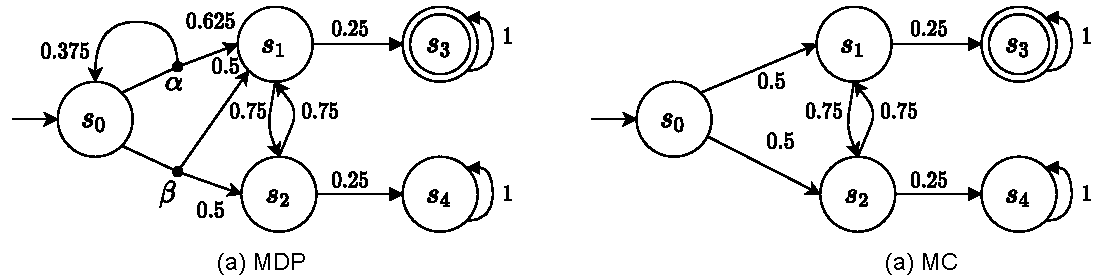
\includegraphics[width=1.0\textwidth]{figures/models.pdf}
\caption{The introduced kinds of probabilistic models \,--\, MDP and MC.}%
\label{fig:models}%
\end{figure*}

\begin{example}[Probabilistic models]
Figure~\ref{fig:param_models} depicts an pMDP and an pMC.
Let us consider the~following valuation $u: \{ x \mapsto 0.5, y \mapsto 0.75 \}$.
By applying this valuation to an~pMDP results in parameter-free MDP depicted at Figure~\ref{fig:models},~and the~same in the~case of MC instantiated from relevant pMC.
\end{example}

Instinctively,~we can imagine an~$MC$ as a~state-transition system with the~following semantics.
A~probability distribution for each state $\forall s \in S: \mathcal{P}(S)$ represents a~stochastic choice of firing the~transition from such state $s \in S$ to one of its successors states $s' \in supp(\mathcal{P(S)})$.
Consequently,~an~$MC$ defined with such semantics has a~\textit{Markov property} (memorylessness), which is essential when modelling systems and for efficient analysis.
This property declares that the~probability of the~transition from state $s \in S$ to state $s' \in supp(\mathcal{P(S)})$ depends only on the~current state,~and it is independent of the~taken path of chain to state $s$.
We can see that each state of an $MC$ disposes of a unique probability distribution over its possible successor states.
MDPs define an~extension of $MCs$ introducing a~non-deterministic choice between several probability distributions over each state.

A~(in)finite sequence $\pi = s_0 \overset{a_0}{\rightarrow} s_1 \overset{a_1}{\rightarrow} \dots$,~where $s_i \in S$,~$a_i \in Act(s_i)$,~and $\mathbb{P}(s_i, a_i)(s_{i+1}) \neq 0$ for all $i \in \mathbb{N}$ represents the~\textit{path} of an~MDP M.
For finite $\pi$, $last(\pi)$ denotes the last state of $\pi$,~and the~set of (in)finite paths of M we denotes as $Paths_{fin}^{M}\,(Paths^M)$.
When an~$MDP$ is currently in the~state $s \in S$,~it has a~non-deterministic choice of an action $a \in Act(s)$ leading to the~one possible probability distribution $\mathcal{P}(s)(a)$ over its successors' states.
These actions cause the~non-deterministic behaviour of an~$MDP$.
Still,~this property can be suppressed by applying a~\textit{scheduler},~which selects one specific action in each state,~i.e.,~transforms an~$MDP$ to an~$MC$.

% \begin{definition}[MDP]
% \cite{roman-DP}
%     A Markov decision process (MDP) $M$ is a~quadruple $\mdp$ ~where $S$ is a~finite set of states,~$s_0 \in S$ is an~initial state,~$Act$ is a~finite set of actions,~and $\mathcal{P}: S \times Act  \nrightarrow Distr(S)$ represents a~(partial) transition probability function. 
% \end{definition}

% A~set $\mathit{Act(s) = \{ a \in Act \; \lvert \; \mathcal{P}(s, a) \neq \; \perp \}}$ for state $s \in S$ represents the~\textit{available} actions.
% When holds $\lvert \mathit{Act(s)} \rvert = 1$ for each state $s \in S$,~such MDP straightforward induces an~MC.

\begin{definition}[Scheduler]
\cite{cegar}
A scheduler for an MDP $M = \mdp$ is a function $\sigma: Paths_{fin}^{M} \rightarrow Act$ such that $\sigma(\pi) \in Act(last(\pi))$ for all $\pi \in Paths_{fin}^{M}$.
Scheduler $\sigma$ is memory-less if $last(\pi) = last(\pi') \Longrightarrow \sigma(\pi) = \sigma(\pi')$ for all $\pi, \pi' \in Paths_{fin}^{M}$.
The set of all schedulers of M is $\Sigma^M$.
\end{definition}

\begin{definition}[Induced MC] \label{def:incuded_mc}
\cite{cegar}
An MC induced by MDP M and $\sigma \in \Sigma^M$ is defined by $M_{\sigma} = ( Paths_{fin}^{M}, s_0, \mathbf{P}^{\sigma})$ where:
\begin{align*}
    \mathbf{P^{\sigma}}(\pi, \pi') = 
    \begin{cases}
        \mathcal{P}(last(\pi), \sigma(\pi))(s') \quad & if \; \pi' = \pi \overset{\sigma(\pi)}{\rightarrow} s' \\
         0 \quad & otherwise.
    \end{cases}
\end{align*}
\end{definition}


\section{Probabilistic Synthesis}
We use a~\textit{sketch}~\cite{sketching1,sygus}, ~which represents a~incomplete high-level description of a~probabilistic system,~to describe the~family of MCs.
It usually describes the~modelled system's fixed behaviour,~but it also contains the~undefined one represented by \textit{holes}.
They represent the~incomplete parts of a~program that must be instantiated so that the~final description satisfies a~given specification.
We note that the~holes correspond to parameters,~and their instantiation yields a~concrete Markov chain.
At follow, we formalise the sketch defining the set of designs:

\begin{definition}[Sketch]
Let $\sketch$ be a~sketch containing holes from the~set $\mathcal{H} = \left\{ H_k \right \}_k$ with $R_k$ being the~set of options available for hole $H_k$.
Let $\rlzf = \prod_k R_k$ denote the~set of all hole assignments (realizations),~$\sketch[r]$ denote the~program induced by a~substitution $r \in \rlzf$ and $\fmlr$ denote the underlying MC.
Note that the~set $\rlzf$ is exponential in $\lvert \mathcal{H} \rvert$.
\end{definition}

\todo{Some description ...}

\begin{definition}[Specification]
In our work,~we focus on the~conjunctions of specifications with \textit{reachability} and \textit{expected rewards}.
Let $T$ be a~set of target states,~then the~reachability property $\varphi \equiv \reachability{\bowtie}{\lambda}{T}$ where $\bowtie \in \{<, \leq, >, \geq\}$ and $0 \leq \lambda \leq 1$ expresses that the~probability of reaching $T$ refers to $\lambda \in [0,1]$ in agreement with $\bowtie$.
Expected reward property $\phi \equiv \reward {\bowtie}{\lambda}{T}$ expresses that the~expected reward accumulated before $T$ is reached refers to $\lambda \in \mathbb{R}^+$ in accordance with $\bowtie \, \in \{<, \leq \}$.
Let $\mathcal{P}[r]$ be a~program induced by the~realisation $r$,~we denote $\mathcal{P}[r] \models \varphi$ when this program satisfies the~specification $\varphi$.
Let $\varPhi = \{ \varphi_i \}_{i \in I}$ be a~finite set of specifications,~when $\forall i \in I: \mathcal{P}[r] \models \varphi_i$ then we write $\mathcal{P}[r] \models \varPhi$.
\end{definition}

We aim to two kinds of synthesis tasks for a~given probabilistic program described with a~realisation set $\rlzf$,~and a~specification set $\varPhi$.
The first task tries to identify just one realisation $r \in \rlzf$ that satisfy the~given specification set $\varPhi$.
This task represents a~special instance of the~threshold synthesis,~which tries to divide the~realisation set $\rlzf$ into two subsets based on their satisfiability.
We do not address this synthesis task in our work.
The second task on which we focus our attention is finding a~realisation that minimises or maximises a~given objective.

\begin{definition}[Feasibility]
Find a realisation $r \in \rlzf$ such that $\mathcal{P}[r] \models \varPhi$. 
\end{definition}

\begin{definition}[Minimality] \label{def:minimality}
For property $\phi_{\min}$, find a realisation $r^* \in \rlzf$ such that:
$$r^* \in \argmin_{r \in \rlzf} \left \{ \prob[\sketch[r] \models \phi_{\max}] \mid \sketch[r] \models \varPhi \right \}.$$.
\end{definition}

We defined only minimal synthesis task for probability property,~but its variants for maximisation and expected rewards may be defined analogously.
Moreover, we focus also to a relaxed variant of minimal synthesis, the so-called \textit{$\varepsilon$-minimal synthesis}, defined as follows: $\mathcal{P}[r^*] \models \varPhi \; and \; 
\mathbb{P}[\mathcal{P}[r^*] \models \varphi_{min}] \leq (1 - \varepsilon) \cdot \min_{r \in \mathcal{\overline{R}}} \{ \mathbb{P}[\mathcal{P}[r] \models \varphi_{min}] \; \lvert \; \mathcal{P}[r] \models \varPhi \}.$

\begin{example} (Synthesis problem)
Assume an~MCs family $\fml$ from Example~\ref{exam:mcfamily} and the~specification $\phi = \reachability{\geq}{0.1}{\{s_1\}}$.
The solution to the~feasibility synthesis problem is,~for example,~the~realisation $r_0$, since $D_{r_0}$ has a~probability of $\frac{2}{3}$ to reach state $s_1$.
For $\varPhi = [F \; \{s1\}]$,~the~solution to the~maximal synthesis problem on MCs family $\fml$ is the~realisation $r_2$,~as MC $D_{r_2}$ has a~probability equal to one to reach state $s_1$.
\end{example}